\documentclass[]{aiaa-tc}% insert '[draft]' option to show overfull boxes

% Zach del Rosario's LaTeX macros, May 2016
% Inspired by Paul Constantine's macros

\usepackage{amsmath} % Needed for \boldsymbol, etc.
\usepackage{amsfonts} % Needed for \mathbb, etc.
\usepackage{graphicx}
\usepackage{mathtools} % Needed for \ceil and \floor
% Break with AIAA template
% \usepackage{caption}
% \usepackage{subcaption}

% Image Macro: \img{filename}{caption}
% \newcommand{\img}[2]{
% 	\begin{figure}[H]
% 	\centering
% 	\includegraphics[width=0.6\textwidth]{../images/#1}   % first argument is the file
% 	\caption{#2}                  % second argument is caption
% 	\label{fig:#1}                % generate label from first argument
% 	\end{figure} }

% Double Image Macro: \img{file1}{file2}{caption1}{caption2}
% \newcommand{\imgtwo}[4]{
% 	\begin{figure}
% 	\centering
% 	\begin{minipage}{.5\textwidth}
% 		\centering
% 		\includegraphics[width=0.9\linewidth]{../images/#1}
% 		\captionof{figure}{#3}
% 		\label{fig:#1}
% 	\end{minipage}%
% 	\begin{minipage}{.5\textwidth}
% 		\centering
% 		\includegraphics[width=0.9\linewidth]{../images/#2}
% 		\captionof{figure}{#4}
% 		\label{fig:#2}
% 	\end{minipage}
% 	\end{figure}
% }

% Table Macro: \tab{filename}{caption}
% \newcommand{\tab}[2]{
% 	\begin{table}[H]
% 	\centering
% 	\input{../tables/#1.tex} 	% first argument is filename
% 	\caption{#2} 				% second argument is caption
% 	\label{tab:#1} 				% generatae label from filename
% 	\end{table}
% }

% Logic
\newcommand{\logeq}{\Leftrightarrow}

% Probability
\newcommand{\E}{\mathbb{E}}

% Index
% Use these in star form; i.e. \floor*{x/2}
\DeclarePairedDelimiter\ceil{\lceil}{\rceil}
\DeclarePairedDelimiter\floor{\lfloor}{\rfloor}

% Vector symbol macros
\newcommand{\vsym}[1]{\boldsymbol{#1}}

\newcommand{\va}{\boldsymbol{a}}
\newcommand{\vb}{\boldsymbol{b}}
\newcommand{\vc}{\boldsymbol{c}}
\newcommand{\vd}{\boldsymbol{d}}
\newcommand{\ve}{\boldsymbol{e}}
\newcommand{\vf}{\boldsymbol{f}}
\newcommand{\vg}{\boldsymbol{g}}
\newcommand{\vh}{\boldsymbol{h}}
\newcommand{\vi}{\boldsymbol{i}}
\newcommand{\vj}{\boldsymbol{j}}
\newcommand{\vk}{\boldsymbol{k}}
\newcommand{\vl}{\boldsymbol{l}}
\newcommand{\vm}{\boldsymbol{m}}
\newcommand{\vn}{\boldsymbol{n}}
\newcommand{\vo}{\boldsymbol{o}}
\newcommand{\vp}{\boldsymbol{p}}
\newcommand{\vq}{\boldsymbol{q}}
\newcommand{\vr}{\boldsymbol{r}}
\newcommand{\vs}{\boldsymbol{s}}
\newcommand{\vt}{\boldsymbol{t}}
\newcommand{\vu}{\boldsymbol{u}}
\newcommand{\vv}{\boldsymbol{v}}
\newcommand{\vw}{\boldsymbol{w}}
\newcommand{\vx}{\boldsymbol{x}}
\newcommand{\vy}{\boldsymbol{y}}
\newcommand{\vz}{\boldsymbol{z}}

% Vector symbol + tilde macros
\newcommand{\vtlm}[1]{\tilde{\boldsymbol{#1}}}

\newcommand{\vta}{\tilde{\boldsymbol{a}}}
\newcommand{\vtb}{\tilde{\boldsymbol{b}}}
\newcommand{\vtc}{\tilde{\boldsymbol{c}}}
\newcommand{\vtd}{\tilde{\boldsymbol{d}}}
\newcommand{\vte}{\tilde{\boldsymbol{e}}}
\newcommand{\vtf}{\tilde{\boldsymbol{f}}}
\newcommand{\vtg}{\tilde{\boldsymbol{g}}}
\newcommand{\vth}{\tilde{\boldsymbol{h}}}
\newcommand{\vti}{\tilde{\boldsymbol{i}}}
\newcommand{\vtj}{\tilde{\boldsymbol{j}}}
\newcommand{\vtk}{\tilde{\boldsymbol{k}}}
\newcommand{\vtl}{\tilde{\boldsymbol{l}}}
\newcommand{\vtm}{\tilde{\boldsymbol{m}}}
\newcommand{\vtn}{\tilde{\boldsymbol{n}}}
\newcommand{\vto}{\tilde{\boldsymbol{o}}}
\newcommand{\vtp}{\tilde{\boldsymbol{p}}}
\newcommand{\vtq}{\tilde{\boldsymbol{q}}}
\newcommand{\vtr}{\tilde{\boldsymbol{r}}}
\newcommand{\vts}{\tilde{\boldsymbol{s}}}
\newcommand{\vtt}{\tilde{\boldsymbol{t}}}
\newcommand{\vtu}{\tilde{\boldsymbol{u}}}
\newcommand{\vtv}{\tilde{\boldsymbol{v}}}
\newcommand{\vtw}{\tilde{\boldsymbol{w}}}
\newcommand{\vtx}{\tilde{\boldsymbol{x}}}
\newcommand{\vty}{\tilde{\boldsymbol{y}}}
\newcommand{\vtz}{\tilde{\boldsymbol{z}}}

% Matrix symbol
\newcommand{\mA}{\boldsymbol{A}}
\newcommand{\mB}{\boldsymbol{B}}
\newcommand{\mC}{\boldsymbol{C}}
\newcommand{\mD}{\boldsymbol{D}}
\newcommand{\mE}{\boldsymbol{E}}
\newcommand{\mF}{\boldsymbol{F}}
\newcommand{\mG}{\boldsymbol{G}}
\newcommand{\mH}{\boldsymbol{H}}
\newcommand{\mI}{\boldsymbol{I}}
\newcommand{\mJ}{\boldsymbol{J}}
\newcommand{\mK}{\boldsymbol{K}}
\newcommand{\mL}{\boldsymbol{L}}
\newcommand{\mM}{\boldsymbol{M}}
\newcommand{\mN}{\boldsymbol{N}}
\newcommand{\mO}{\boldsymbol{O}}
\newcommand{\mP}{\boldsymbol{P}}
\newcommand{\mQ}{\boldsymbol{Q}}
\newcommand{\mR}{\boldsymbol{R}}
\newcommand{\mS}{\boldsymbol{S}}
\newcommand{\mT}{\boldsymbol{T}}
\newcommand{\mU}{\boldsymbol{U}}
\newcommand{\mV}{\boldsymbol{V}}
\newcommand{\mW}{\boldsymbol{W}}
\newcommand{\mX}{\boldsymbol{X}}
\newcommand{\mY}{\boldsymbol{Y}}
\newcommand{\mZ}{\boldsymbol{Z}}

 \usepackage{varioref}%  smart page, figure, table, and equation referencing
 \usepackage{wrapfig}%   wrap figures/tables in text (i.e., Di Vinci style)
 \usepackage{threeparttable}% tables with footnotes
 \usepackage{dcolumn}%   decimal-aligned tabular math columns
  \newcolumntype{d}{D{.}{.}{-1}}
 \usepackage{nomencl}%   nomenclature generation via makeindex
  \makenomenclature
 \usepackage{subfigure}% subcaptions for subfigures
 \usepackage{subfigmat}% matrices of similar subfigures, aka small mulitples
 \usepackage{fancyvrb}%  extended verbatim environments
  \fvset{fontsize=\footnotesize,xleftmargin=2em}
 \usepackage{lettrine}%  dropped capital letter at beginning of paragraph
 % \usepackage[dvips]{dropping}% alternative dropped capital package
 \usepackage[colorlinks]{hyperref}%  hyperlinks [must be loaded after dropping]
 \usepackage{booktabs} % for \toprule and \bottomrule

 \title{Pursuing Active Manifolds via Nonlinear Optimization}

 \author{
  Zachary R. del Rosario\thanks{PhD Candidate, Aeronautics and Astronautics, 496 Lomita Mall, Stanford CA, AIAA Student Member.}\\
  {\normalsize\itshape
   Stanford University, Stanford CA, 94305, USA}\\
 }

 % Data used by 'handcarry' option
 % \AIAApapernumber{YEAR-NUMBER}
 % \AIAAconference{Conference Name, Date, and Location}
 % \AIAAcopyright{\AIAAcopyrightD{YEAR}}

 % Define commands to assure consistent treatment throughout document
 \newcommand{\eqnref}[1]{(\ref{#1})}
 \newcommand{\class}[1]{\texttt{#1}}
 \newcommand{\package}[1]{\texttt{#1}}
 \newcommand{\file}[1]{\texttt{#1}}
 \newcommand{\BibTeX}{\textsc{Bib}\TeX}

 % Define document-specific shortcuts
 \newcommand{\dom}{\mathcal{D}}

\begin{document}

\maketitle

\begin{abstract}
Dimension Reduction is an approach to alleviating the Curse of Dimensionality. Active Subspaces is a dimension reduction technique which seeks linear subspaces which are `active'; that is, they capture the majority of variation in some quantity of interest (QoI). While useful in practice, Active Subspaces do not always exist. A natural generalization is to seek \emph{Active Manifolds}, curved spaces which capture variations in our QoI. The problem of finding Active Manifolds is posed here as a nonlinear optimization problem, and solved using interior point methods.
\end{abstract}

\printnomenclature % creates nomenclature section produced by MakeIndex

%-------------------------------------------------
\section{Introduction} \label{sec:introduction}
%-------------------------------------------------

\lettrine[nindent=0pt]{O}{ne} of the most challenging difficulties facing high-fidelity modeling is the treatment of high-dimensional parameter spaces: the Curse of Dimensionality. Consider a parameter study on some quantity of interest (QoI) $f$ in a space $\dom\subseteq\mathbb{R}^m$; a simple heuristic is to use $10$ points per dimension, in order to well represent the parameter space. Then the total number of sample points is $10^m$. If a computer code implementing our model executes in a fixed time of $1$ second, then our parameter study execution time scales exponentially. Figure \ref{fig:curse_of_dimensionality} depicts the aforementioned scenario.
\nomenclature{$\dom$}{Domain of $f$}%

The only reasonable strategy to mitigate this challenge is to perform \emph{dimension reduction}, that is, to reduce $m$. One scheme for dimension reduction of this sort is to seek \emph{Active Subspaces} -- linear subspaces in parameter space along which the majority of variation in our QoI is captured. \cite{constantine2015} The Active Subspaces approach gives a `perfect' dimension reduction in the case that our QoI is a Ridge Function; that is, for $\vx\in\mathbb{R}^m$ and $\mA\in\mathbb{R}^{m\times k}$ with $k<m$, we have $f(\vx)=g(\mA^T\vx)$. Note that a Ridge Function is constant along directions which are orthogonal to $\mA$, that is

\begin{equation}
\mW^T\nabla f = 0 \logeq \mW^TA = 0, \label{eq:ridge_property}
\end{equation}

where $\nabla f$ is the gradient of $f$, understood to be a column vector. One example of a Ridge Function is $f(\vx) = \frac{1}{2}(.7x_1+.3x_2)^2$. In this case, the Active Subspace approach discovers the Active and Inactive directions, depicted in Figure \ref{fig:as_example}. Note that this gives us a `perfect' dimension reduction, as we can completely neglect changes along the direction $[-.3,.7]^T$. Such Ridge Functions may seem like a contrivance, but they are actually quite common in multivariate Fourier Transforms\cite{pinkus2015} and physical laws in general.\cite{Constantine2016} Nevertheless, Ridge Functions are not the only functional form that arises in practice; in this case the Active Subspace is approximate. While approximate Active Subspaces are useful, it is easy to construct functions which do not admit this sort of low-dimensional structure, even in an approximate sense. In these cases, we would like to do more than simply give up.

\begin{wrapfigure}{R}{0.5\linewidth}
 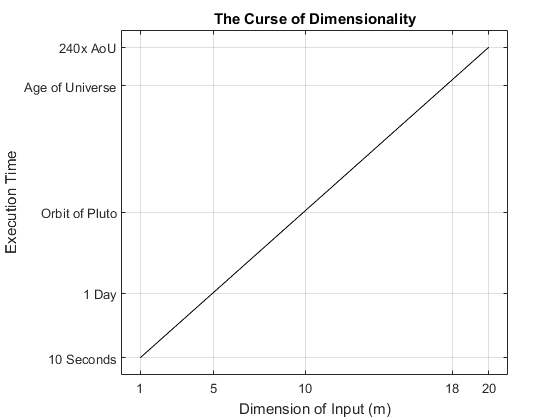
\includegraphics{../images/curse_of_dimensionality}
 \caption{Execution time scales exponentially with the dimension of parameter space.}
 \label{fig:curse_of_dimensionality}
\end{wrapfigure}

A natural generalization of Active Subspaces is to seek \emph{Active Manifolds}; that is, curved subsets of parameter space which capture the variability of a function. Such low-dimensional structures should recover linear subspaces in the case that they exist (i.e. a Ridge Function), and more general spaces when they do not. Note that if a function is differentiable, we can always move along the gradient to capture the full variability of a function -- unfortunately this requires perfect knowledge of the function, which brings us back to the Curse of Dimensionality. In practice we must use a limited number of gradient samples (assumed to be available, say through an adjoint solution\cite{Jameson1988} or automatic differentiation\cite{Rall1981}) to numerically approximate such a manifold.

\begin{wrapfigure}{R}{1.0\linewidth}
 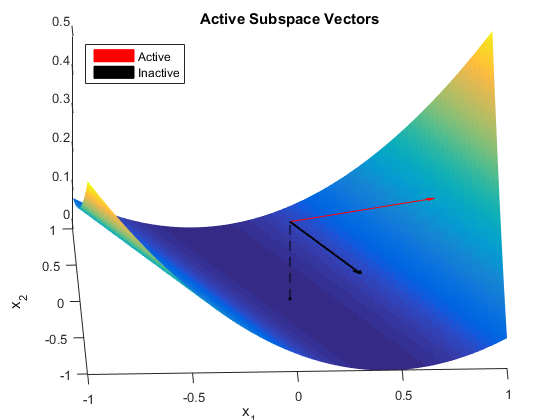
\includegraphics{../images/surface_plot}
 \caption{Note that on average, the function changes more along the active directions than the inactive directions; in this case, the change in the inactive direction is exactly zero.}
 \label{fig:as_example}
\end{wrapfigure}

In this work, we focus on the \emph{identification} of Active Manifolds, and leave their usage to subsequent works. The re-parameterization of a function on an Active Subspace is already laden with important considerations, which is further complicated by generalization to more arbitrary spaces. These are important issues which lie outside the scope of this document.

%-------------------------------------------------
\section{Seeking Active Manifolds} \label{sec:active_manifolds}
%-------------------------------------------------
The strategy we will adopt in this work is to generalize the properties of a Ridge Function: By allowing Equation \ref{eq:ridge_property} to vary in space, we arrive at

\begin{equation}
  \label{eq:inactive_manifold}
  \mW(\vx)^T \nabla f(\vx) = 0.
\end{equation}%
\nomenclature{$\vx$}{Input vector}%
\nomenclature{$f(\vx)$}{Scalar quantity of interest}%
\nomenclature{$\nabla f(\vx)$}{Gradient of QoI}%
\nomenclature{$\mW(\vx)$}{Manifold matrix}%

Equation \ref{eq:inactive_manifold} gives us a set of directions $\mW(\vx)$ along which $f(\vx)$ does not vary -- these directions define \emph{Inactive Manifolds}, while the orthogonal directions define \emph{Active Manifolds}. Note that as long as $f(\vx)$ is differentiable, we know $\mW(\vx)$ exists, as we can simply perform a QR decomposition on the $m\times m$ identity matrix, augmented with $\nabla f$. While this is mathematically possible, such a scheme is computationally intractable due to being an infinite dimensional problem. Instead, we must settle on a finite dimensional problem by approximating Equation \ref{eq:inactive_manifold}.

First, we will consider a single direction $\vw_j(\vx)$, and parameterize on a finite number of basis functions. Choose a set of $k$ differentiable functions $\phi_i:\mathbb{R}^m\to\mathbb{R}$, and set

\begin{equation}
\label{eq:parameterized_w}
\vw_j(\vx) = \sum_{i=1}^k \alpha_{ij}\nabla\phi_i(\vx),
\end{equation}
\nomenclature{$\vw_j(\vx)$}{Manifold vector}%
\nomenclature{$\vsym{\alpha}_j$}{Manifold parameter vector}%
\nomenclature{$\phi_i$}{Manifold basis function}%
\nomenclature{$k$}{Number of basis functions}%

where the $\alpha_{ij}$ parameterize $\vw_j(\vx)$ in a linear fashion. Now we construct $\mW(\vx)$ from a collection of these $\vw_j(\vx)$, each parameterized on a different $\vsym{\alpha}_j$ vector, that is

\begin{equation}
\mW(\vx) = [\vw_1(\vx),\dots,\vw_l(\vx)].
\end{equation}

Rather than attempt to solve for $\mW$ all at once, we will attempt to enforce Equation \ref{eq:inactive_manifold} for each $\vw_j(\vx)$ individually. We must make two concessions though. First, even though the $\vw_j$ are now parameterized on a finite set, Equation \ref{eq:inactive_manifold} is enforced at all points $\vx\in\dom$: In practice we must sample a number of points $\{\vx_i\}_{i=1}^n\subseteq\dom$ and enforce $\vw_j^T(\vx_i)\nabla f(\vx_i)=0$ on this set. Second, unless $\mW$ lies precisely within the span of the $\nabla\phi_i$, Equation \ref{eq:inactive_manifold} will hold only approximately: In practice we will attempt to minimize the residual, defined by
\nomenclature{$n$}{Number of sample points in $\dom$}%

\begin{equation}
\label{eq:residual}
R = \|\mM\vsym{\alpha}\|_2,
\end{equation}

where

\begin{equation}
\label{eq:matrix_m}
\mM = \left[\begin{array}{ccc}%
    \nabla\phi_1^T(\vx_1)\nabla f(\vx_1) & \cdots & \nabla\phi_k^T(\vx_1)\nabla f(\vx_1) \\
    \vdots & \ddots & \vdots \\
    \nabla\phi_1^T(\vx_n)\nabla f(\vx_n) & \cdots & \nabla\phi_k^T(\vx_n)\nabla f(\vx_n) \\
    \end{array}\right].
\end{equation}

Note that if $\mM\vsym{\alpha}=0$, then Equation \ref{eq:inactive_manifold} holds exactly for $\mW=[\vw]$, parameterized on $\vsym{\alpha}$. Also note that this fixed $\mM$ defines the residual for each $\vw_j$, as they are each parameterized on the same basis, albeit with a different $\vsym{\alpha}$. Na{\"i}vely, we may seek to minimize the residual $R$ directly; however, this optimization problem has a trivial solution $\vsym{\alpha}=0$. In practice we constrain the length via $\|\vsym{\alpha}\|_2\geq1$. Additionally, note that we wish to solve for a \emph{collection} of $\vsym{\alpha}_j$; we can accomplish this by demanding that each new $\vsym{\alpha}_j$ be orthogonal to the previous ones. Finally, we add a 1-norm term to encourage sparsity; we would like each $\vsym{\alpha}_i$ to be `simple', in the sense of being sparse. This leads to the following sequence of optimization problems

\begin{equation}
\begin{aligned}
\label{eq:optimization}
\text{min  }& \|\mM\vsym{\alpha}_j\|_2 + \beta\|\vsym{\alpha}_j\|_1, \\
\text{s.t. }& \|\vsym{\alpha}_j\|_2\geq1, \\
            & \mA_j^T \vsym{\alpha}_j = 0,
\end{aligned}
\end{equation}

where $\beta>0$ is a tunable weighting parameter, and $\mA_j=[\vsym{\alpha}_1,\dots,\vsym{\alpha}_{j-1}]$, with $\mA_1=0$. There are a few important points to note: First, one should sovle Problem \ref{eq:optimization} a number of times equal to the number of Inactive Manifolds sought -- one could either define a fixed number of manifolds to seek, or continue running until the residual cannot be reduced under some desired tolerance. The former method is appropriate if the degree of dimension reduction required is already known, while the latter will discover the maximum reduction available, subject to the choice of basis. Second, Problem \ref{eq:optimization} has a convex objective function but a nonlinear constraint, thus we do \emph{not} enjoy the benefits of a convex problem. This creates issues when attempting to design a solver, which will be addressed in Section \ref{sec:solver}\ref{sec:solver_design}.

%------------------------
\subsection{Choice of Basis} \label{sec:basis}
The choice of basis functions $\phi_i$ is crucial for obtaining an Active Manifold. The basis must be chosen to include $\mW(\vx)$, at least in some approximate sense. In the case of a Ridge Function the Active Manifolds are linear subspaces, so a linear choice of basis $\phi_i(\vx) = x_i$ is appropriate. In fact, choosing a linear basis and approximating Equation \ref{eq:inactive_manifold} by finding the nullspace via a Singular Value Decomposition (SVD) exactly recovers the Active Subspace procedure! To see this, substitute the linear basis into Equation \ref{eq:matrix_m} to find

\begin{equation}
\label{eq:matrix_m_linear}
\mM_l = [\nabla f(\vx_1),\dots,\nabla f(\vx_n)]^T.
\end{equation}

Equation \ref{eq:inactive_manifold} corresponds to the condition $\mM_l\vsym{\alpha}=0$, which is a nullspace computation. This can be accomplished by considering the SVD of $\mM_l=U\Sigma V^T$; the vectors $\vv_i$ which correspond to the zero singular values $\sigma_i$ form a basis for the nullspace of $\mM_l$. These are found via an eigenvalue decomposition of $\mM_l^T\mM_l$, which equals

\begin{equation}
\label{eq:sum_m}
\mM_l^T\mM_l = \sum_{i=1}^n \nabla f(x_i) \nabla f^T(x_i).
\end{equation}

Note that the Active Subspace is also found via an eigenvalue decomposition of the $\mC$ matrix, defined as the weighted average of the outer product of the gradient.\cite{constantine2015} Compare Equation \ref{eq:sum_m} to the Monte Carlo approximation of the $\mC$ matrix

\begin{equation}
\label{eq:sum_c}
\hat{\mC} = \frac{1}{n} \sum_{i=1}^n \nabla f(x_i) \nabla f^T(x_i).
\end{equation}

Note that up to a factor of $n$, they are the same! Thus, for the correct choice of basis, the Active Manifold procedure defined above should recover Active Subspaces. This is important, as it shows that if our basis is chosen correctly and Problem \ref{eq:optimization} approximates Equation \ref{eq:inactive_manifold} well, we can do no worse than Active Subspaces.

In this work, we try a number of different sets of basis functions, defined in Table \ref{tab:basis} below. These include both the linear basis and larger sets.

\begin{table}
\centering
\begin{tabular}{ll}
\toprule
Name & Basis \\
\midrule
Linear & $x_i$ \\
Quadratic & $x_i$, $x_i^2$, $\log(|x_i|)$ \\
Cubic & $x_i$, $x_i^2$, $x_i^3$, $\log(|x_i|)$, $x_i^{-1}$ \\
\bottomrule
\end{tabular}
\caption{Basis sets used in numerical experiments.}
\label{tab:basis}
\end{table}

%-------------------------------------------------
\section{Solver} \label{sec:solver}
%-------------------------------------------------
In order to solve Problem \ref{eq:optimization}, a nonlinear solver was designed, implemented, and tested on a number of different quantities of interest $f$ and sets of basis functions $\phi_i$.

%------------------------
\subsection{Solver Design} \label{sec:solver_design}
As mentioned in Section \ref{sec:active_manifolds}, the optimization problem in question is a nonlinear optimization problem with nonlinear constraints. The solver is an implementation of the interior point method using log-barrier functions and a quasi-Newton method using the BFGS update rule.\cite{Chandrupatla1999} In this scheme, we first solve the feasibility problem by constructing an objective function on the constraints, then run the interior point method successively relaxing the barriers.

Note that one could construct a log-barrier on the linear constraint $\mA^T_j\vsym{\alpha}_j=0$. Instead, we employ \emph{progressive reparameterization}; that is, reparameterizing the problem such that the constraint is automatically satisfied. We accomplish this for step $j$ by constructing a set of vectors $[\vtq_{1j},\dots,\vtq_{k-j+1}]=\tilde{\mQ}_j$ orthogonal to all previous solutions $[\vsym{\alpha}_1,\dots,\vsym{\alpha}_{j-1}]=\mA_j$, and defining a new set of $k-j+1$ variables $\vtlm{\alpha}_j$ which replace the old $\vsym{\alpha}_j=\tilde{\mQ}_j\vtlm{\alpha}_j$. Note that by this construction $\vsym{\alpha}_j$ is orthogonal to all previous solutions.

Note that the first iteration $j=1$ of Problem \ref{eq:optimization} has no linear constraint, so the solver described above is sufficient. For subsequent iterations, we redefine the variables as described above and optimize over $\vtlm{\alpha}_j$. Our new optimization problem is

\begin{equation}
\begin{aligned}
\label{eq:optimization_reparam}
\text{min  }& \|\mM\tilde{\mQ}_j\vtlm{\alpha}_j\|_2 + \beta\|\tilde{\mQ}_j\vtlm{\alpha}_j\|_1, \\
\text{s.t. }& \|\tilde{\mQ}_j\vtlm{\alpha}_j\|_2\geq1,
\end{aligned}
\end{equation}

where $\vtlm{\alpha}\in\mathbb{R}^{k-j+1}$, and $\tilde{\mQ}_j$ is found by taking the last $k-j+1$ columns of the orthogonal matrix found from an economy QR decomposition of $\mA_j$, augmeted with the $k\times k$ identity matrix

\begin{equation}
\label{eq:augmeted_matrix}
[\mA_j,\mI] = \mQ\mR.
\end{equation}

Note that since the QR decomposition has a complexity of $O(n^3)$, this method is inappropriate for excessively high-dimensional spaces. In these cases, it may be prudent to approximate the linear constraint with a barrier function. However, it is worth noting that since the computational cost we are trying to alleviate is exponential, a cubic cost may still be comparatively cheap.

Finally, we must address the lack of convexity in our optimization problem. Problem \ref{eq:optimization} is non-convex, and thus may contain local minima. This is problematic with our interior point method, which for a poor choice of initial guess may converge to such a local optimum. To alleviate this issue, we employ a restart heuristic: We begin with a uniform random guess within a unit box in the positive orthant, and if at any stage $j$ the residual (Eq. \ref{eq:residual}) does not drop below an absolute threshold, we restart that stage with a new initial guess. This is an admittedly simple solution, which is not guaranteed to solve the problem, but it works well enough in practice.

%------------------------
\subsection{Solver Performance} \label{sec:solver_performance}

% Convergence in Residual

% Comparison against Active Subspaces for Ridge Function

% Comparison against AS for quadratic function

%-------------------------------------------------
\section{Conclusion} \label{sec:conclusion}
%-------------------------------------------------

Concluding remarks, yo.

% produces the bibliography section when processed by BibTeX
\bibliography{bibtex_database}
\bibliographystyle{aiaa}

\end{document}

% - Release $Name:  $ -
